\documentclass[tikz,border=8pt]{standalone}
\usetikzlibrary{arrows.meta,positioning,calc}
\begin{document}
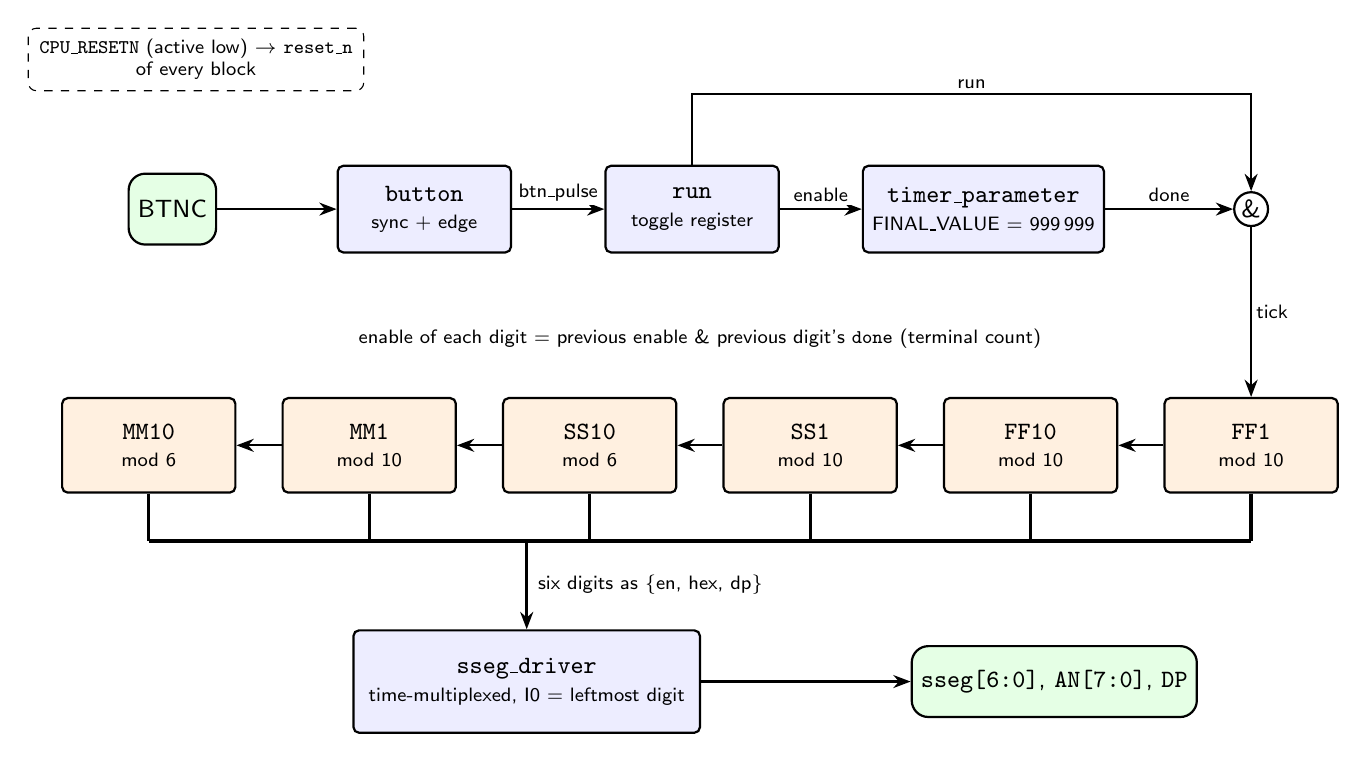
\begin{tikzpicture}[
    font=\sffamily\small,
    >={Stealth[length=2.2mm]},
    blk/.style={draw, thick, rounded corners=2pt, minimum height=1.1cm, minimum width=2.2cm, align=center, fill=blue!7},
    io/.style={draw, thick, rounded corners=6pt, minimum height=0.9cm, align=center, fill=green!10},
    cnt/.style={draw, thick, rounded corners=2pt, minimum height=1.2cm, minimum width=2.2cm, align=center, fill=orange!12},
    gate/.style={draw, thick, circle, inner sep=1pt, fill=white},
    lbl/.style={font=\sffamily\scriptsize, inner sep=1.5pt, fill=white},
    wire/.style={thick, ->},
    bus/.style={very thick, ->}
]
% ---------- row 1: control (left to right) ----------
\node[io]  (btnc)  at (0,6)    {BTNC};
\node[blk] (btn)   at (3.2,6)  {\texttt{button}\\[-1pt]\scriptsize sync + edge};
\node[blk] (run)   at (6.6,6)  {\texttt{run}\\[-1pt]\scriptsize toggle register};
\node[blk] (timer) at (10.3,6) {\texttt{timer\_parameter}\\[-1pt]\scriptsize FINAL\_VALUE = 999\,999};
\node[gate](tick)  at (13.7,6) {\&};

\draw[wire] (btnc) -- (btn);
\draw[wire] (btn) -- node[lbl,above=1pt]{btn\_pulse} (run);
\draw[wire] (run) -- node[lbl,above=1pt]{enable} (timer);
\draw[wire] (timer) -- node[lbl,above=1pt]{done} (tick);
\draw[wire] (run.north) -- ++(0,0.9) -| node[lbl,pos=0.25,above]{run} (tick.north);

% ---------- row 2: digit chain (right to left) ----------
\node[cnt] (ff1)  at (13.7,3) {\texttt{FF1}\\[-1pt]\scriptsize mod 10};
\node[cnt] (ff10) at (10.9,3) {\texttt{FF10}\\[-1pt]\scriptsize mod 10};
\node[cnt] (ss1)  at (8.1,3)  {\texttt{SS1}\\[-1pt]\scriptsize mod 10};
\node[cnt] (ss10) at (5.3,3)  {\texttt{SS10}\\[-1pt]\scriptsize mod 6};
\node[cnt] (mm1)  at (2.5,3)  {\texttt{MM1}\\[-1pt]\scriptsize mod 10};
\node[cnt] (mm10) at (-0.3,3) {\texttt{MM10}\\[-1pt]\scriptsize mod 6};

\draw[wire] (tick.south) -- node[lbl,right]{tick} (ff1.north);
\draw[wire] (ff1)  -- (ff10);
\draw[wire] (ff10) -- (ss1);
\draw[wire] (ss1)  -- (ss10);
\draw[wire] (ss10) -- (mm1);
\draw[wire] (mm1)  -- (mm10);
\node[lbl, fill=none] at (6.7,4.35)
    {enable of each digit = previous enable \& previous digit's \texttt{done} (terminal count)};

% ---------- row 3: display ----------
\draw[very thick] (mm10.south) -- ++(0,-0.6) coordinate(b1);
\foreach \n in {mm1,ss10,ss1,ff10,ff1}{\draw[very thick] (\n.south) -- ++(0,-0.6);}
\draw[very thick] (b1) -- ($(ff1.south)+(0,-0.6)$);

\node[blk, minimum width=4.4cm, minimum height=1.3cm] (disp) at (4.5,0)
    {\texttt{sseg\_driver}\\[-1pt]\scriptsize time-multiplexed, I0 = leftmost digit};
\draw[bus] (4.5,1.8) -- node[lbl,right=2pt]{six digits as \{en, hex, dp\}} (disp.north);
\node[io, minimum width=3.6cm] (outs) at (11.2,0) {\texttt{sseg[6:0]}, \texttt{AN[7:0]}, \texttt{DP}};
\draw[wire] (disp) -- (outs);

% ---------- reset note ----------
\node[draw, dashed, rounded corners=3pt, align=center, font=\sffamily\scriptsize, inner sep=4pt]
    at (0.3,7.9) {\texttt{CPU\_RESETN} (active low) $\rightarrow$ \texttt{reset\_n}\\of every block};
\end{tikzpicture}
\end{document}
